\selectlanguage{english}
\clearpage
\section{Design and Automation of Tests}

This chapter presents the design and implementation of a test system focused on \textbf{integration testing} of the eCAL middleware. In integration tests, multiple components or subsystems are combined and tested as a group to verify that they interact correctly. This is especially relevant for communication middleware, where the interaction between distributed publishers, subscribers, servers, and clients must be validated under real-world conditions.

\vspace{0.9em}
The primary goal is to evaluate eCAL’s behavior in realistic scenarios involving inter-process communication across various transport mechanisms. To achieve this, a container based test infrastructure was created that allows isolated, repeatable, and automated execution of test cases. The infrastructure combines Robot Framework for test orchestration with Docker for process isolation, fault simulation, and reproducibility.

\vspace{0.9em}
The test environment targets publish-subscribe and RPC-based communication patterns and includes both normal operation and fault scenarios (e.g., process crashes or network failures). All tests are designed as integration tests and verify the end-to-end behavior of communicating components rather than isolated units.

\vspace{0.9em}
The structure of this chapter is as follows: Section 5.1 introduces the test environment and its components. Section 5.2 details the infrastructure and core implementation elements. Section 5.3 explains how edge cases and failure scenarios are handled. Section 5.4 presents selected test cases along with their validation logic. Section 5.5 explains the automation of test execution and how it integrates with a CI/CD pipeline. Section 5.6 describes the visualization of test results via web-based reports. Finally, Section 5.7 provides a summary of the findings and key insights.

\subsection{Test Environment Overview}

To enable structured and reproducible integration testing of the eCAL middleware, a dedicated test environment was designed. It is based on containerized execution using Docker and orchestrated by Robot Framework. Each test case runs in isolation, supports custom configurations, and can simulate both normal and faulty communication behavior.

\vspace{1em}
The test suite is structured to maximize modularity and clarity. Each scenario resides in a self-contained folder that includes the necessary C++ binaries, test logic, and scripts for container orchestration. Common libraries and configuration helpers are maintained separately to support reuse and consistency across all test cases.

\subsubsection*{Folder Layout and Test Case Assets}

The integration test repository follows a modular layout. Each test case resides in its own folder and contains its specific C++ components, test definitions, and build logic. Shared helper libraries and the base image are placed separately. An overview is provided below in Listing~\ref{lst:folder_structure}:

\vspace{0.5em}
\begin{lstlisting}[basicstyle=\ttfamily\small, frame=single, caption={Simplified directory structure with key contents}, captionpos=b, label={lst:folder_structure}]
 integration_tests/
 +-- <test_case>/              # Example: basic_pub_sub/
 |  +-- src/                   # C++ sources
 |  |  +-- publisher.cpp       # Publishes test messages
 |  |  +-- subscriber.cpp      # Receives messages
 |  |  +-- CMakeLists.txt      # Build definition
 |  |
 |  +-- robottests/
 |  |  +-- <test_case>.robot   # Test logic
 |  +-- scripts/
 |  |  +-- build_images.sh     # Builds test container
 |  |  +-- entrypoint.sh       # Launches test role 
 |  |                            (pub/sub)
 |  +-- docker/
 |     +-- Dockerfile          # Test-specific image
 |  
 +-- lib/
 |  +-- EcalConfigHelper/      # C++ helpers
 |  +-- DockerLibrary.py       # Keywords for docker
 |  +-- GlobalPathsLibrary.py  # Folder and naming 
 |                               utilities
 +-- docker/
 |  +-- Dockerfile.ecal_base   # Base image for all tests
 ----
 create_new_test/              # Generator for new tests
\end{lstlisting}

This structure supports automation and reuse. New test cases can be added easily by following the same layout. A generator tool is provided to ensure consistency when creating new folders and test assets.


\vspace{1.5em}
Each folder, as shown in the structure above, forms the foundation for a complete integration test. However, the layout alone does not reflect how the test logic is executed across tools and containers. To better understand this process, the following diagrams explain the test flow in practice: from orchestrating the test logic with Robot Framework to running binaries inside Docker containers.

\vspace{1em}
In particular, the next two views illustrate (1) the execution flow of a typical test case and (2) the container architecture used to simulate different communication modes. The test infrastructure supports both \textit{network-based} and \textit{local communication}. 

\vspace{1em}
\subsubsection*{1. Execution Flow of a Test Case}

\begin{figure}[H]
	\centering
	\includegraphics[width=0.36\textwidth]{Images/test_execution_flow.png}
	\caption{Execution flow of an integration test: Robot Framework initiates the build, launches containers, collects results, and generates reports.}
	\label{fig:ecal_test_execution_flow}
\end{figure}

The test process begins with Robot Framework triggering a build script that compiles and packages the necessary eCAL binaries into Docker containers. These containers are then launched with appropriate runtime parameters and network configuration. Once started, the container's \texttt{entrypoint.sh} script executes the actual test binary (e.g., publisher or subscriber), which performs the communication logic. 

\vspace{1em}
After test execution, Robot Framework collects logs, inspects exit codes, and generates structured reports. This entire process is fully automated and ensures reproducibility across multiple test runs.

\vspace{1em}
Figure~\ref{fig:ecal_test_execution_flow} illustrates the step-by-step execution of an integration test, including all involved components and their responsibilities.

\vspace{1em}
\subsubsection*{2. Container Architecture: Network vs. Local Mode}

\begin{figure}[H]
	\centering
	\includegraphics[width=0.9\textwidth]{Images/test_architecture_diagram3.png}
	\caption{Container architecture for test execution: left side shows network-based separation with inter-container communication; right side shows a single container with both roles for local testing.}
	\label{fig:ecal_container_architecture}
\end{figure}

Depending on the selected communication mode, eCAL nodes are either distributed across multiple containers (network mode) or run together inside a single container (local mode). 

\vspace{1em}
In \textbf{network mode}, each component (e.g., publisher and subscriber) runs in a dedicated container. These containers are connected via a virtual Docker network that allows UDP or TCP communication across IP boundaries. This setup reflects realistic inter-process communication in distributed systems.

\vspace{1em}
In \textbf{local mode}, both publisher and subscriber are launched inside a single container. Communication takes place entirely within the container, allowing use of shared memory (SHM) or local UDP/TCP transport layers. This configuration is ideal for verifying behavior in tightly coupled systems without involving external network interfaces.

\vspace{1em}
Figure~\ref{fig:ecal_container_architecture} shows the two setup variants side by side.

\vspace{1em}
This flexible design allows for testing a wide range of scenarios, including those where communication modes must be explicitly selected or changed during runtime. The environment also allows easy simulation of errors, such as killing a process, disconnecting a network, or injecting delays, which are critical for the validation of robustness. All implementations are maintained in the public repository \texttt{ecal-test-suite}~\cite{ecal_test_suite_repo}.

\subsection{Implementation of the Test Infrastructure}

The integration test infrastructure for eCAL was designed to be modular, reusable, and easy to extend. It allows new test cases to be added or removed quickly by following a consistent folder structure and execution pattern. This is particularly useful for one of the most common use cases in test driven development: adding a new test scenario with minimal overhead.

\vspace{1em}
In addition, the infrastructure supports isolated and repeatable testing by combining Docker-based execution with Robot Framework-based test definitions. To improve clarity and maintainability, the system is structured into shared infrastructure components and test specific scripts. The following subsections provide an overview of these elements.

\vspace{1em}
The interaction and execution flow of the test system, from Robot Framework orchestration to container-level execution and evaluation, is illustrated in Figure~\ref{fig:ecal_test_flow}.



\begin{landscape}
	\clearscrheadings
	\ofoot{}
	
	\begin{figure}[H]
		\centering
		\includegraphics[width=1.41\textwidth]{Images/ecal_test_flow.png}
		\caption{Test flow for eCAL-based integration testing}
		\label{fig:ecal_test_flow}
	\end{figure}
\end{landscape}

\clearpage
\pagestyle{scrheadings}


Figure~\ref{fig:ecal_test_flow} illustrates the complete execution flow of the eCAL integration test system. At the top, individual Docker containers host separate eCAL components such as publishers and subscribers, each launched via an \texttt{entrypoint.sh} script that starts the corresponding C++ application. These containers are connected via a virtual Docker network to enable inter-process communication.

\vspace{1em}
The entire container setup is managed by the Robot Framework, which coordinates test execution, container startup, and fault injection (e.g., network disconnects). During runtime, logs and exit codes are collected by Robot Framework and evaluated to determine test outcomes. The final results are stored in a structured format and exported for further analysis. This layered architecture ensures reproducibility, isolation, and full control over test execution and validation.

\subsubsection*{5.2.1 Shared Infrastructure Components}

The core logic for container orchestration and test coordination is encapsulated in reusable libraries and helper utilities. These components are used across all test cases and form the foundation of the test environment.

\vspace{1em}
\textbf{1. DockerLibrary.py}

\vspace{0.3em}
This custom Python library for Robot Framework provides keywords to manage Docker containers. It simplifies the interaction with Docker by offering reusable commands that can be used directly in test cases. The library hides complex details and enables clear and reliable test automation.

\vspace{0.5em}
Some of the main features of the DockerLibrary are:

\begin{itemize}
	\item \textbf{Starting and stopping containers:} Containers can be launched with custom names, arguments, or even fixed IP addresses if needed.
	\item \textbf{Log collection:} Output from running containers is collected and made available for test evaluation and debugging.
	\item \textbf{Exit code handling:} The library waits for the container to finish and reads its exit code to determine if the test passed or failed.
	\item \textbf{Network control:} Containers can be connected to or disconnected from Docker networks during the test, allowing the simulation of network failures.
	\item \textbf{Container tracking:} Containers are stored in memory using unique names, so they can be easily referenced and stopped later in the test.
	\item \textbf{Error handling:} If a container has already been removed or cannot be found, a warning is shown instead of causing a crash.
\end{itemize}

\vspace{0.5em}
A common use case is stopping and cleaning up test containers after the test has finished. Listing~\ref{lst:docker_py_stop} shows a simplified version of the \texttt{Stop Container} keyword in Python, while Listing~\ref{lst:docker_robot_stop} shows how this keyword is used in a Robot Framework test case.

\vspace{1em}
\begin{lstlisting}[style=cppstyle, language=Python, caption={Example keyword implementation in \texttt{DockerLibrary.py}}, label={lst:docker_py_stop}, captionpos=b]
 @keyword
 def stop_container(self, name):
     if name in self.containers:
        try:
           self.containers[name].stop()
           self.containers[name].remove()
        except NotFound:
           BuiltIn().log_to_console(f"Container {name} already removed.")
        finally:
           self.containers.pop(name, None)
\end{lstlisting}

\vspace{0.5em}
\begin{lstlisting}[style=cppstyle, caption={Calling \texttt{Stop Container} in a Robot Framework test}, label={lst:docker_robot_stop}, captionpos=b]
 *** Settings ***
 Library           lib/DockerLibrary.py	
 
 *** Test Cases ***
 Start Test
 Start Container    my_test_container
 
 ---Test Implementation here---  
 
 Cleanup After Test
 Stop Container    my_test_container
\end{lstlisting}

\vspace{1em}
\textbf{2. GlobalPathsLibrary.py}

\vspace{0.3em}
This library handles dynamic path and tag resolution across all test modules. It defines the active test case, provides access to configuration scripts, and ensures that Docker image names, container labels, and result folders are consistently named and resolved.

\clearpage
\vspace{1em}
\textbf{3. ecal\_config\_helper.h / .cpp}

\vspace{0.3em}
This shared C*+ utility is responsible for configuring communication parameters such as transport mode and layer activation. It includes two central helper functions:

\begin{itemize}
	\item \texttt{wait\_for\_subscriber()} – ensures that messages are only published once a subscriber is available (see Listing~\ref{lst:wait_for_subscriber}).
	\item \texttt{setup\_ecal\_configuration()} – configures the desired communication mode (e.g., UDP, TCP, SHM) for each process (see Listing~\ref{lst:setup_ecal}).
\end{itemize}

\begin{lstlisting}[style=cppstyle, caption={Simplified wait\_for\_subscriber logic}, label={lst:wait_for_subscriber}, captionpos=b]
 void wait_for_subscriber(std::string topic){
   while (!has_subscriber(topic)){
     sleep_for(std::chrono::milliseconds(100));
   }
 }
\end{lstlisting}

\vspace{1em}
\begin{lstlisting}[style=cppstyle, caption={Partial example for UDP setup}, label={lst:setup_ecal}, captionpos=b]
 if (mode == "local_udp"){
    config.communication_mode = 
    eCAL::eCommunicationMode::local;
    if (is_publisher){
    	config.publisher.layer_priority_local = 
    	{eCAL::TransportLayer::udp_mc};
    } else {
    	config.subscriber.layer.shm.enable = false;
    	config.subscriber.layer.udp.enable = true;
    	config.subscriber.layer.tcp.enable = false;
    }
 }
\end{lstlisting}

\clearpage
\subsubsection*{5.2.2 Test Structure and Scripts}

Each test case in the integration test suite is placed in a separate folder and follows a consistent internal structure. This organization ensures modularity and supports clean separation between infrastructure logic and test specific behavior. Most test folders include the following components:

\vspace{1em}
\textbf{1. Test Definitions and Assets}

\vspace{0.3em}
Each test case is defined by a Robot Framework file (e.g., \texttt{network\_crash.robot}) that describes the test logic in a readable and structured format. These test definitions make use of high-level keywords such as \texttt{Start Container}, \texttt{Disconnect Container}, or \texttt{Validate Payload} to coordinate the setup, execution, and verification of each scenario. The Robot file serves as the central control layer for the test case and interacts with the supporting infrastructure components.

\vspace{1em}
\textbf{2. build\_images.sh}

\vspace{0.3em}
This shell script is used to build the Docker images required for the test case. It typically invokes CMake to compile the C++ binaries (e.g., publishers, subscribers, or RPC clients/servers) and packages them with the necessary configuration and helper scripts. Since each test case may include custom logic or message types, the build process is isolated per test case. This enables reproducibility and prevents interference between different tests. Furthermore, the script tags each image with a unique label, which supports traceability in CI pipelines.

\vspace{1em}
\textbf{3. entrypoint.sh}

\vspace{0.3em}
This script is executed as the container's entry point and is responsible for launching the correct binary with the appropriate arguments. Depending on the test case, it may select the role (e.g., publisher, subscriber), set the communication mode, start multiple processes, or coordinate test-specific timing behavior. Each test provides its own version of this script, tailored to the scenario being validated.


\subsubsection*{5.2.3 Automated Test Case Generation}

To simplify the creation of new test cases and ensure consistency across the test suite, a Python-based code generation tool was developed. This script uses the \texttt{Jinja2} templating engine to automatically create a fully structured test folder, including predefined files such as Robot Framework test definitions, C++ source files, build scripts, and configuration templates.

\vspace{1em}
The tool is invoked via the command line and takes a single argument – the name of the new test case. Based on this input, it generates all required files and inserts the correct identifiers and filenames using placeholders defined in the Jinja2 templates. This ensures that the generated test case follows the expected naming conventions and folder hierarchy without manual adjustments.

\vspace{1em}
In addition to rendering the file content, the tool automatically creates the directory structure and marks relevant shell scripts (e.g., \texttt{build\_images.sh}, \texttt{entrypoint.sh}) as executable. Each file includes commented placeholders or example logic to guide further development.

\vspace{1em}
The use of templated test generation reduces repetitive setup work and improves maintainability. It also supports onboarding by making it easier to add new test cases without requiring in-depth knowledge of the full infrastructure. The template logic can be adapted or extended as needed and is located in a separate \texttt{templates/} directory within the project. The generator tool and all template definitions are maintained in the public repository of the eCAL test suite~\cite{ecal_test_generator, ecal_test_suite_repo}.


\vspace{1em}
\subsubsection*{5.2.4 Summary}

The test infrastructure is structured to separate reusable core logic from test-specific implementations. Shared libraries handle Docker orchestration, dynamic path management, and transport configuration. Test case folders contain all relevant scripts, test logic, and compiled binaries in a self-contained structure. This design ensures that new scenarios can be added with minimal overhead while maintaining consistency and reproducibility.

\vspace{1em}
To further support extensibility and reduce manual setup effort, a generator tool based on Jinja2 templates was developed. It automates the creation of new test cases by producing a complete and consistent folder structure, including example content and executable scripts. This significantly improves maintainability, speeds up onboarding, and supports systematic test development.

\clearpage
\subsection{Handling of Edge Cases}

A key requirement for testing communication middleware is the ability to validate system behavior under abnormal or unexpected conditions. Distributed systems are inherently prone to failures, such as delayed messages, process crashes, or temporary network interruptions. Therefore, in addition to verifying functional correctness, the test environment must support controlled simulation of such conditions.

\vspace{1em}
This section introduces the strategies used to simulate and evaluate edge cases and fault scenarios within the automated test infrastructure. The goal is to uncover potential weaknesses in eCAL’s communication logic and validate its resilience.

\vspace{1em}
\textbf{Fault Injection Capabilities}

\vspace{0.4em}
To enable realistic fault simulations, the Robot Framework infrastructure supports fault injection mechanisms:

\begin{itemize}
	\item \textbf{Crash simulation:} Docker containers running eCAL nodes can be stopped manually during the test to simulate process crashes.
	\item \textbf{Network disconnection:} Containers can be detached from their virtual Docker network at runtime to mimic network cable unplug or wireless dropout.
	\item \textbf{Network reconnection:} Containers can be reconnected to the network after a delay, allowing tests to evaluate recovery behavior and reconnection logic.
	\item \textbf{Delays and timeouts:} Artificial delays are injected using sleep commands or slow message loops, which help simulate jitter or processing backpressure.
\end{itemize}

These mechanisms are reusable and can be invoked in any test scenario. For example, Listing~\ref{lst:rf_disconnect_example} shows how a network disconnect and reconnect is triggered inside a Robot Framework test case:

\vspace{0.5em}
\begin{lstlisting}[style=cppstyle, caption={Simulating a temporary network disconnect and reconnect}, label={lst:rf_disconnect_example}, captionpos=b]
 Disconnect Container From Network   test_client   ecal_net
 Sleep    6s
 Reconnect Container   test_client   ecal_net  ip=172.28.0.10
\end{lstlisting}

\vspace{1em}
\textbf{Observed Edge Case Categories}

\vspace{0.4em}
The following edge case categories were explicitly targeted in test scenarios:

\begin{itemize}
	\item \textbf{Missing receivers:} Publishers start sending before any subscribers are active. These tests confirm that no blocking or crashes occur and that late subscribers still receive messages once available.
	
	\item \textbf{Message loss and recovery:} By crashing publishers or subscribers mid-test, message loss is deliberately introduced. The system’s ability to continue communicating correctly with the remaining nodes is then evaluated.
	
	\item \textbf{Reconnect scenarios:} Clients or servers are disconnected from the network and reconnected after a delay. These tests assess whether communication can be re-established without restarting the processes.
	
	\item \textbf{Large message handling:} Tests involving very large payloads (e.g., 50\,MB) are used to verify memory usage and crash behavior, especially under Zero-Copy Shared Memory configurations.
\end{itemize}

\vspace{0.5em}
\textbf{Validation Methods}

\vspace{0.4em}
To verify correct behavior during and after edge conditions, the following evaluation strategies are used:

\begin{itemize}
	\item \textbf{Exit code checks:} Each component returns an exit code indicating success or failure. Robot Framework interprets these codes to determine whether the test passed.
	
	\item \textbf{Payload inspection:} Received messages are validated for correctness (e.g., expected values like 42, 43, 44) and assigned to the correct source based on payload content.
	
	\item \textbf{Log analysis:} All container logs are automatically collected and printed in the test report. This helps identify at which point failures occurred and what internal state was reached.
\end{itemize}

\vspace{0.5em}
\textbf{Conclusion and Role in Test Design}

\vspace{0.4em}
The ability to inject faults and simulate edge cases is a central part of the overall test strategy. It ensures that communication logic is not only functionally correct but also resilient under stress and partial failure. Many of the following test cases build directly on these capabilities, combining normal communication with injected disconnects or crash conditions. This approach helps create a realistic, production-like test environment that increases confidence in system stability and fault tolerance.


\subsection{Test Case Design}

This section presents selected integration test cases that were implemented to validate the behavior and robustness of the eCAL middleware. The tests are executed using Robot Framework and Docker-based containers, building upon the infrastructure described in Section~5.2. Each test targets a specific aspect of IPC such as message delivery, fault handling, or service requests and follows a consistent structure in terms of execution and evaluation.

\vspace{1em}
To provide a clearer overview, the test cases are grouped into two categories:

\begin{itemize}
	\item \textbf{Normal Operation Scenarios}: Tests that verify the expected behavior of the middleware under standard conditions.
	\item \textbf{Fault Injection Scenarios}: Tests that simulate failure situations such as process crashes or network disconnects.
\end{itemize}

\vspace{0.3em}
Table~\ref{tab:test_case_overview} summarizes all implemented test cases, including their classification and main focus.
\begin{table}[H]
	\renewcommand{\arraystretch}{1.45}
	\setlength{\tabcolsep}{10pt}
	\centering
	\begin{tabular}{|c|l|l|}
		\hline
		\textbf{ID} & \textbf{Title} & \textbf{Type} \\
		\hline
		\textbf{\hyperref[sec:tc1]{TC 1}} & \textbf{\hyperref[sec:tc1]{Publisher to Subscriber}} & Normal Operation \\
		\hline
		\textbf{\hyperref[sec:tc2]{TC 2}} & \textbf{\hyperref[sec:tc2]{Multiple Publishers/Subscribers}} & Normal Operation \\
		\hline
		\textbf{\hyperref[sec:tc3]{TC 3}} & \textbf{\hyperref[sec:tc3]{RPC Ping Request-Response}} & Normal Operation \\
		\hline
		\textbf{\hyperref[sec:tc4]{TC 4}} & \textbf{\hyperref[sec:tc4]{RPC N:N Communication}} & Normal Operation \\
		\hline
		\textbf{\hyperref[sec:tc5]{TC 5}} & \textbf{\hyperref[sec:tc5]{Publisher Crash (in Transmission)}} & Fault Injection \\
		\hline
		\textbf{\hyperref[sec:tc6]{TC 6}} & \textbf{\hyperref[sec:tc6]{Subscriber Crash (in Reception)}} & Fault Injection \\
		\hline
		\textbf{\hyperref[sec:tc7]{TC 7}} & \textbf{\hyperref[sec:tc7]{Network Failure Simulation}} & Fault Injection \\
		\hline
		\textbf{\hyperref[sec:tc8]{TC 8}} & \textbf{\hyperref[sec:tc8]{RPC Reconnect (Network Failure)}} & Fault Injection \\
		\hline
	\end{tabular}
	\caption{Overview of test cases and their classification}
	\label{tab:test_case_overview}
\end{table}

Each test case includes a description of its objective, execution flow, success criteria, configuration details, and an evaluation of the observed results.  In addition, code examples are provided to illustrate relevant implementation details, including how publishers, subscribers, or RPC clients are configured and how data is processed. The next subsections present the individual test cases in detail.

\vspace{1em}
\subsubsection{Test Case 1: Publisher to Subscriber Communication}
\label{sec:tc1}
\textbf{Objective:}

\vspace{0.4em}
Ensure that a message published by a single publisher is reliably received by a single subscriber using a specific transport layer (e.g., shared memory, TCP or UDP) (see Table~\ref{tab:basic_comm_test}).

\vspace{0.5em}
\textbf{Execution:}
\begin{itemize}
	\item In local modes (e.g., \texttt{local shm}, \texttt{local udp}), the publisher and subscriber run inside a single container.
	\item In network modes (e.g., \texttt{network udp}, \texttt{network tcp}), the publisher and subscriber run in separate containers connected via a Docker network.
	\item The publisher sends a small binary payload of value \texttt{42} (repeated) and logs each send event.
	\item The subscriber listens on the topic, logs received values, and exits successfully if the expected messages were received within the timeout window.
\end{itemize}

\textbf{Success Criteria:}
\begin{itemize}
	\item Subscriber receives 100\,\% of all messages sent.
	\item No crashes or communication timeouts occur.
	\item The subscriber exits with return code \texttt{0}.
\end{itemize}

\begin{table}[H]
	\centering
	\begin{tabular}{@{}llll@{}}
		\toprule
		\textbf{Component} & \textbf{Role} & \textbf{Transport Mode} & \textbf{Payload} \\
		\midrule
		basic\_pub  & Publisher  & All Modes  & \texttt{0x2A} (42) \\
		basic\_sub  & Subscriber & All Modes  & 42 \\
		\bottomrule
	\end{tabular}
	\caption{Configuration for Basic Communication Test}
	\captionsetup{position=bottom}
	\label{tab:basic_comm_test}
\end{table}


\textbf{Code Examples:}

\vspace{0.4em}
To illustrate key aspects of the basic communication test, the following code excerpts highlight how the publisher and subscriber are implemented.

\vspace{1em}
The publisher creates a binary buffer of size 10 where each byte is set to \texttt{0x2A} (decimal 42). This value is used consistently across all test scenarios to simplify result verification (see Listing \ref{lst:basic_pub_send}).

\vspace{1em}
The subscriber callback reads the first byte of the received buffer and casts it to an integer. This ensures that the payload can be easily validated (see Listing \ref{lst:basic_sub_receive}).
\vspace{0.5em}

\begin{lstlisting}[style=cppstyle, caption={Binary buffer with value 42 used by the publisher}, label={lst:basic_pub_send}, captionpos=b]
 std::vector<unsigned char> buffer(10, 42);
 pub.Send(buffer.data(), buffer.size());
\end{lstlisting}

\begin{lstlisting}[style=cppstyle, caption={Extracting first byte from the received message in subscriber}, label={lst:basic_sub_receive}, captionpos=b]
 int value = static_cast<int>(
 static_cast<const unsigned char*>(data_.buffer)[0]
 );
\end{lstlisting}

\begin{lstlisting}[style=cppstyle, caption={Argument setup using TCLAP in both publisher and subscriber}, label={lst:tclap_basic}, captionpos=b]
 TCLAP::ValueArg<std::string> mode_arg(
 "m", "mode", "Transport mode", true, "", "string");
 
 TCLAP::ValueArg<std::string> topic_arg(
 "t", "topic", "Topic name", false, "test_topic", "string");
 
 TCLAP::ValueArg<std::string> name_arg(
 "n", "name", "eCAL node name", false, "pub_test", "string");
 
 TCLAP::ValueArg<int> count_arg(
 "c", "count", "Number of messages", false, 3, "int");
 
 TCLAP::ValueArg<int> delay_arg(
 "d", "delay", "Delay between sends", false, 1000, "int");
\end{lstlisting}

\vspace{0.4em}
The configuration with TLCAP in Listing \ref{lst:tclap_basic} allows full flexibility for running the same binary with different roles and transport modes. The \texttt{--mode} parameter (e.g., \texttt{local\_tcp}) enables switching between eCAL transport layers without modifying the code. The use of TCP is especially useful for tests that simulate network scenarios across Docker containers, where shared memory is not applicable.

\vspace{1em}

\textbf{Evaluation:}

\vspace{0.4em}
This basic test confirms that eCAL reliably delivers messages across all supported transport modes under ideal conditions. The results show that communication remains consistent in both local and networked setups, provided the configuration parameters are correctly applied. This test serves as the foundation for more advanced scenarios such as crash handling, message validation, or multi-topic communication.


\vspace{1em}
\vspace{1em}
\subsubsection{Test Case 2: Multiple Publishers and Subscribers}
\label{sec:tc2}

\textbf{Objective:}

\vspace{0.4em}
Verify that multiple publishers can send distinct payloads on the same topic and that multiple subscribers can receive both streams reliably.

\vspace{0.5em}
\textbf{Execution:}
\begin{itemize}
	\item Two publishers send different payloads (42 and 43) on the same topic.
	\item Two subscribers listen to the same topic and count how many messages they receive for each value.
	\item All four nodes run either in a single container (local mode) or separate containers connected via Docker network (network mode).
\end{itemize}

\textbf{Success Criteria:}
\begin{itemize}
	\item Each subscriber receives 100\,\% of the messages from both publishers.
	\item No crash or message loss occurs during transmission.
	\item All containers exit with return code \texttt{0}.
\end{itemize}

\begin{table}[H]
	\centering
	\begin{tabular}{@{}llll@{}}
		\toprule
		\textbf{Component}     & \textbf{Role}    & \textbf{Transport Mode} & \textbf{Payload} \\
		\midrule
		multi\_publisher       & Publisher        & All Modes               & \texttt{0x2B} (43) \\
		multi\_publisher2      & Publisher        & All Modes               & \texttt{0x2A} (42) \\
		multi\_subscriber      & Subscriber       & All Modes               & Both              \\
		multi\_subscriber2     & Subscriber       & All Modes               & Both              \\
		\bottomrule
	\end{tabular}
	\caption{Configuration for Multi-Publisher and Multi-Subscriber Test}
	\label{tab:multi_pub_sub_test}
\end{table}

\textbf{Code Examples:}
\vspace{0.4em}

Listing~\ref{lst:multi_pub1_send} shows how \texttt{multi\_publisher} sends a binary payload containing value 43. Listing~\ref{lst:multi_pub2_send} illustrates the second publisher, which uses value 42. Both publishers send 15 messages with a 1000\,ms delay between sends.
\vspace{0.5em}
\begin{lstlisting}[style=cppstyle, caption={Publisher 1 sends 0x2B (43)}, label={lst:multi_pub1_send}, captionpos=b]
 std::vector<unsigned char> buffer(10, 43);
 pub.Send(buffer.data(), buffer.size());
\end{lstlisting}
\vspace{0.5em}
\begin{lstlisting}[style=cppstyle, caption={Publisher 2 sends 0x2A (42)}, label={lst:multi_pub2_send}, captionpos=b]
 std::vector<unsigned char> buffer(10, 42);
 pub.Send(buffer.data(), buffer.size());
\end{lstlisting}

Each subscriber uses a callback function that increments counters depending on the first byte received. The values 42 and 43 are tracked separately (see Listing~\ref{lst:multi_sub_receive}).
\vspace{0.5em}
\begin{lstlisting}[style=cppstyle, caption={Subscriber callback counting 42 and 43}, label={lst:multi_sub_receive}, captionpos=b]
 if (value == 42) ++count_42;
 if (value == 43) ++count_43;
\end{lstlisting}

\vspace{0.5em}
\textbf{Evaluation:}

\vspace{0.4em}
This test confirms that eCAL supports N:N communication over a shared topic. Both subscribers successfully received messages from both publishers in all tested transport modes. This demonstrates the middleware's ability to handle concurrent sources and destinations. This is a critical feature for scenarios involving aggregation, monitoring, or distributed decision-making.

\vspace{1em}
From a combinatorial perspective, a complete evaluation of the publish-subscribe model would require testing all communication patterns: one-to-one (1:1), one-to-many (1:N), many-to-one (N:1), and many-to-many (N:N). In practice, however, N:N scenarios inherently cover the functional aspects of both 1:N and N:1 communication patterns. This is because every N:N test includes multiple publishers and subscribers and therefore implicitly verifies the correctness of message delivery from one to many (1:N) and from many to one (N:1) within the same execution.

\vspace{1em}
By implementing N:N tests across all five eCAL transport modes (\texttt{local\_shm}, \texttt{local\_udp}, \texttt{local\_tcp}, \texttt{network\_udp}, \texttt{network\_tcp}), we effectively validate the core functionality and robustness of the middleware under realistic and complex conditions. This strategic reduction in test permutations allows for efficient validation without sacrificing coverage.

\newpage
\subsubsection{Test Case 3: RPC Ping Request-Response}
\label{sec:tc3}

\textbf{Objective:}

\vspace{0.4em}
Verify that a client can successfully call a remote method ("Ping") on an eCAL RPC server and receive a valid response.

\vspace{0.5em}
\textbf{Execution:}
\begin{itemize}
	\item The \texttt{rpc\_ping\_server} registers a service method named \texttt{Ping}.
	\item The \texttt{rpc\_ping\_client} connects to the server and sends a request with content \texttt{"PING"}.
	\item The server responds with \texttt{"PONG"}.
	\item The client validates the response and exits with code \texttt{0}.
\end{itemize}

\textbf{Success Criteria:}
\begin{itemize}
	\item The server receives and processes a request.
	\item The response string \texttt{"PONG"} is printed by the client.
	\item The client exits with return code \texttt{0}.
\end{itemize}

\begin{table}[H]
	\centering
	\begin{tabular}{@{}lllll@{}}
		\toprule
		\textbf{Component} & \textbf{Role} & \textbf{Mode} & \textbf{Method} & \textbf{Expected Response} \\
		\midrule
		rpc\_ping\_server  & RPC Server   & network\_udp & Ping & PONG \\
		rpc\_ping\_client  & RPC Client   & network\_udp & Ping & PONG \\
		\bottomrule
	\end{tabular}
	\caption{Configuration for RPC Ping Test}
	\label{tab:rpc_ping_test}
\end{table}


\textbf{Code Examples:}

\vspace{0.4em}
The server registers a method named \texttt{Ping} that responds with \texttt{PONG} if it receives \texttt{PING} as request (Listing~\ref{lst:rpc_n_n_server_callback}).

\begin{lstlisting}[style=cppstyle, caption={RPC Server handler for method "Ping"}, label={lst:rpc_n_n_server_callback}, captionpos=b]
 server.SetMethodCallback(method_info, [](const eCAL::
 SServiceMethodInformation&, const std::string& request,
 std::string& response) -> int {
   if (request == "PING"){
     response = "PONG";
     return 0;
   }
   response = "UNKNOWN";
   return 1;
 });
\end{lstlisting}

The client connects to the server, sends \texttt{"PING"}, waits for the reply, and prints the server’s response (Listing~\ref{lst:rpc_client_call}).

\begin{lstlisting}[style=cppstyle, caption={RPC Client sends Ping request and prints response}, label={lst:rpc_client_call}, captionpos=b]
 std::string request = "PING";
 std::vector<eCAL::SServiceResponse> responses;
 bool success = client.CallWithResponse("Ping", request, responses, 1000);
	
 for (const auto& response : responses){
   std::cout << "[Client] Server response: " << response.response << std::endl;
 }
\end{lstlisting}

\vspace{0.5em}
\textbf{Evaluation:}

\vspace{0.4em}
This test verifies the correct implementation of eCAL’s RPC interface using a request–response pattern. It confirms that the client and server can communicate over UDP using named service methods. The use of response validation and exit codes allows automated checking of RPC behavior in CI pipelines. It also shows how clients can discover services and call remote methods in a distributed testing environment using Docker and Robot Framework.

\subsubsection{Test Case 4: RPC N:N Communication}
\label{sec:tc4}

\textbf{Objective:}

\vspace{0.4em}
Verify that multiple clients can simultaneously call the same RPC method on multiple eCAL servers and receive a valid response. This test evaluates the scalability and correctness of eCAL’s service-based communication pattern under N:N conditions.

\vspace{0.5em}
\textbf{Execution:}
\begin{itemize}
	\item Two RPC servers register a service named \texttt{rpc\_n\_to\_n\_service} with the method \texttt{Ping}.
	\item Each of the two clients connects to all available servers and sends a \texttt{"PING"} request.
	\item Each server responds with \texttt{"PONG"}.
	\item Each client verifies the number and content of responses and exits with return code \texttt{0}.
\end{itemize}

\newpage

\vspace{0.4em}
\textbf{Success Criteria:}
\begin{itemize}
	\item All clients receive two responses, each containing \texttt{"PONG"}.
	\item No timeout or connection errors occur.
	\item All clients exit with return code \texttt{0}.
\end{itemize}

\vspace{0.4em}
\begin{table}[H]
	\centering
	\begin{tabular}{@{}lllll@{}}
		\toprule
		\textbf{Component} & \textbf{Role} & \textbf{Count} & \textbf{Mode} & \textbf{Expected Response} \\
		\midrule
		rpc\_n\_to\_n\_server & RPC Server & 2 & network\_udp & PONG \\
		rpc\_n\_to\_n\_client & RPC Client & 2 & network\_udp & 2×PONG \\
		\bottomrule
	\end{tabular}
	\caption{Configuration for RPC N:N Communication Test}
	\label{tab:rpc_n_n_test}
\end{table}

\vspace{0.5em}
\textbf{Code Examples:}

The client sends a Ping request and validates that all received responses are equal to \texttt{"PONG"} (Listing~\ref{lst:rpc_n_n_client_response}).

\begin{lstlisting}[style=cppstyle, caption={RPC Client receives multiple responses}, label={lst:rpc_n_n_client_response}, captionpos=b]
 std::vector<eCAL::SServiceResponse> responses;
 client.CallWithResponse("Ping", "PING", responses, 2000);
 int pong_count = 0;
	
 for (const auto& r : responses){
     if (r.response == "PONG") ++pong_count;
 }
 
 return pong_count == 2 ? 0 : 1;
\end{lstlisting}

\vspace{0.4em}
\textbf{Evaluation:}

\vspace{0.4em}
This test confirms that eCAL supports concurrent N:N RPC communication and that multiple clients can address multiple servers via shared service names. It demonstrates that clients receive multiple valid responses for a single call and can handle those responses correctly in parallel scenarios. The test also confirms that the middleware’s internal discovery and routing logic is robust across multiple service providers.

\vspace{1em}
From a test design perspective, this N:N scenario verifies both 1:N and N:1 communication patterns. Each client must discover and contact multiple servers (1:N), and each server must respond correctly to multiple clients (N:1). By executing this test case, the core mechanisms of eCAL's RPC handling are validated across all relevant communication directions, while reducing the total number of required test permutations.

\subsubsection{Test Case 5: Publisher Crash During Transmission}
\label{sec:tc5}

\textbf{Objective:} 

\vspace{0.4em}
Evaluate the system's resilience when one publisher crashes mid-transmission, and ensure that the subscriber still receives messages from the remaining active publisher.

\vspace{0.5em}
\textbf{Execution:}
\begin{itemize}
	\item Two publishers are started: one sends \texttt{42} and crashes after 10 messages, the other sends \texttt{43} continuously.
	\item One subscriber is launched to receive messages from both.
	\item The test runs in all communication modes (local and network).
	\item The subscriber counts messages from both publishers and exits after a fixed timeout.
\end{itemize}

\textbf{Success Criteria:}
\begin{itemize}
	\item The subscriber receives at least 25 messages with value \texttt{43}.
	\item The number of \texttt{42} messages is below the crash threshold (between 5 and 11).
	\item The subscriber exits with return code \texttt{0}.
\end{itemize}

\begin{table}[H]
	\centering
	\begin{tabular}{@{}llll@{}}
		\toprule
		\textbf{Component} & \textbf{Role}     & \textbf{Transport Mode} & \textbf{Payload} \\
		\midrule
		crash\_pub         & Publisher         & All Modes               & \texttt{0x2A} (42) \\
		test\_pub          & Publisher         & All Modes               & \texttt{0x2B} (43) \\
		test\_sub          & Subscriber        & All Modes               & 42 + 43 \\
		\bottomrule
	\end{tabular}
	\caption{Configuration for Crash Resilience Test}
	\label{tab:crash_resilience}
\end{table}

\vspace{0.5em}

\textbf{Code Examples:}

\vspace{0.4em}
The crashing publisher sends a few messages and then exits by calling \texttt{std::abort()}, simulating a runtime failure (Listing~\ref{lst:crash_pub_send}). Meanwhile, the test publisher continues normal operation (Listing~\ref{lst:test_pub_send}).

\vspace{0.5em}
\begin{lstlisting}[style=cppstyle, caption={Crash publisher sends and exits after 10 messages}, label={lst:crash_pub_send}, captionpos=b]
 for (int i = 0; i < total_arg.getValue(); ++i){
  pub.Send(buf.data(), buf.size());
  sleep_for(delay_ms);
  if (i == crash_at_arg.getValue()){
   std::abort();  // Simulate crash
  }
 }
\end{lstlisting}
\vspace{0.5em}
\begin{lstlisting}[style=cppstyle, caption={Resilient publisher continues sending messages}, label={lst:test_pub_send}, captionpos=b]
 for (int i = 0; i < count && eCAL::Ok(); ++i){
  pub.Send(buffer.data(), buffer.size());
  sleep_for(delay_ms);
 }
\end{lstlisting}

The subscriber counts received values and returns 0 only if enough \texttt{43} values are seen and no unexpected continuation from the crashed publisher occurs (Listing~\ref{lst:crash_sub_eval}).

\vspace{0.5em}
\begin{lstlisting}[style=cppstyle, caption={Subscriber decision logic}, label={lst:crash_sub_eval}, captionpos=b]
 if (count_43 >= 25 && count_42 < 11 && count_42 > 4){
   return 0; // Success: resilient communication
 }else{
   return 1; // Failure: not enough or unexpected data
 }
\end{lstlisting}

\vspace{0.5em}

\textbf{Evaluation:}

This test demonstrates that eCAL remains fully functional and continues to deliver messages even when one of the publishers crashes unexpectedly. The second publisher, which sends payload \texttt{43}, continues to operate without interruption. This confirms that the failure of one communication node does not affect the functionality of others. The test was executed in all supported eCAL transport modes, showing that this reliability is consistent regardless of the communication layer.

\vspace{1em}

The use of a crash publisher simulates real world process failures, and the test verifies that message delivery remains uninterrupted. By comparing the message counts, the system ensures that no "phantom" messages are received after the crash point. This approach can be used as a template for testing fault tolerance in distributed IPC systems.

\vspace{1em}
\subsubsection{Test Case 6: Subscriber Crash During Reception}
\label{sec:tc6}

\textbf{Objective:} \\
Verify that the communication remains stable even when one subscriber crashes while receiving large messages.

\vspace{0.5em}
\textbf{Execution:}
\begin{itemize}
	\item A \texttt{large\_publisher} sends three large messages (each about 50\,MB) on the same topic.
	\item One \texttt{crash\_subscriber} is configured to crash after a short time during message reception.
	\item One \texttt{test\_subscriber} continues running and should receive all messages correctly.
	\item The test is executed in all supported eCAL transport modes, except for UDP which cannot handle large messages.
	\item A special variant uses SHM with \texttt{zero\_copy\_mode = true} to verify robustness of shared memory access.
\end{itemize}

\textbf{Success Criteria:}
\begin{itemize}
	\item The stable subscriber exits with return code \texttt{0} and logs successful message reception.
	\item The crashing subscriber terminates due to a simulated failure after a few seconds.
	\item The publisher completes message delivery without interruption or failure.
	\item In SHM mode with Zero-Copy, shared memory corruption or deadlocks must not occur.
\end{itemize}

\begin{table}[H]
	\centering
	\begin{tabular}{@{}llll@{}}
		\toprule
		\textbf{Component} & \textbf{Role}       & \textbf{Transport Mode} & \textbf{Payload} \\
		\midrule
		large\_publisher   & Publisher           & All Modes               & $\sim$50\,MB     \\
		crash\_subscriber  & Subscriber (crash)  & All Modes               & $\sim$50\,MB     \\
		test\_subscriber   & Subscriber (stable) & All Modes               & $\sim$50\,MB     \\
		\bottomrule
	\end{tabular}
	\caption{Configuration for Crash During Reception Test}
	\label{tab:sub_crash_receive}
\end{table}

\vspace{0.5em}
\textbf{Code Example:}

\vspace{0.4em}
The crashing subscriber aborts its process intentionally after two seconds of runtime if it receives any message (see Listing~\ref{lst:sub_crash_logic}).

\begin{lstlisting}[style=cppstyle, caption={Crash condition inside subscriber receive callback}, label={lst:sub_crash_logic}, captionpos=b]
 void OnReceive(
    const eCAL::STopicId&, const eCAL::SDataTypeInformation&,
    const eCAL::SReceiveCallbackData& data_)
 {
  std::cout << "[Crash_Sub] Received " 
  << data_.buffer_size << " bytes\n";
    		
  if (elapsedtime >= 2) {
   std::cerr << "[Crash_Sub] Simulating crash after 2 sec";
   std::abort();
  }
 }

\end{lstlisting}

To simulate high-throughput conditions, the publisher sends three 50\,MB messages and logs each transmission result (see Listing~\ref{lst:large_pub_send}).

\begin{lstlisting}[style=cppstyle, caption={Large message publisher with send confirmation}, label={lst:large_pub_send}, captionpos=b]
 std::string buffer(50L * 1024L * 1024L, 'X');
 for (int i = 0; i < count; ++i){
   bool sent = pub.Send(buffer.data(), buffer.size());
   std::cout << "[Publisher] Send result: " 
             << (sent ? "pass" : "fail");
 }
\end{lstlisting}

\vspace{0.5em}

\textbf{Evaluation:}

\vspace{0.4em}
This test confirms that eCAL maintains stable communication even when a subscriber crashes during the reception of a large message. In all tested configurations except the Zero-Copy SHM variant, the system behaved as expected: the publisher completed its transmission successfully, and the stable subscriber received all messages without interruption. The crash was isolated to the failing subscriber, indicating proper error containment and robustness of the communication layer.

\vspace{1em}
The variant using Zero-Copy in Shared Memory mode highlighted a specific weakness in fault isolation. In Zero-Copy mode, the publisher shares direct memory access with subscribers, which eliminates the need for memory copying and significantly improves performance in high-throughput scenarios. However, this optimization also introduces a stronger coupling between processes at the memory level.

\vspace{1em}
If a subscriber crashes while holding a pointer to shared memory, the publisher (or other subscribers) may experience access violations, resource locks, or inconsistent memory states. This was observed during the test: although the publisher attempted to continue sending data, the shared memory segment could no longer be accessed safely once the crashing subscriber aborted during callback execution. 

\vspace{1em}
Therefore, while Zero-Copy SHM offers performance advantages, it requires careful handling in fault-tolerant systems. Mechanisms such as memory fencing, process monitoring, or fallback copy modes should be considered if system resilience is a priority.

\vspace{1em}
In conclusion, this test underscores both the reliability of eCAL in standard SHM, TCP, and UDP scenarios and the current limitations when using Zero-Copy SHM without additional safeguards. Future testing or deployment scenarios should carefully consider the trade-off between performance and fault tolerance when using advanced features like Zero-Copy.

\vspace{1em}
\subsubsection{Test Case 7: Network Failure Simulation}
\label{sec:tc7}

\textbf{Objective:}

\vspace{0.4em}
Verify that after a simulated network failure, a new local UDP publisher can be successfully launched and establish communication with a running local UDP subscriber. This simulates a scenario where a redundant or backup component becomes active only after failure detection.

\vspace{0.5em}
\textbf{Execution:}
\begin{itemize}
	\item \textbf{Phase 1:} A local UDP publisher (\texttt{local\_publisher\_1}) and a subscriber run in the same container. The publisher sends payloads with value 42.
	\item \textbf{Phase 2:} A network UDP publisher (\texttt{network\_publisher}) runs in a separate container and sends payloads with value 43.
	\item \textbf{Phase 3:} After 7 seconds, the \texttt{network\_publisher} container is disconnected from the Docker network to simulate a network cable unplug.
	\item \textbf{Phase 4:} A second local UDP publisher (\texttt{local\_publisher\_2}) is started within the original container after a short delay. It sends payloads with value 44.
	\item The subscriber logs received values and verifies all expected transitions.
\end{itemize}

\vspace{0.4em}
\textbf{Success Criteria:}
\begin{itemize}
	\item Subscriber receives:
	\begin{itemize}
		\item All sent messages with value 42 (from local\_publisher\_1).
		\item At least 2 messages with value 43 (before network disconnection).
		\item All sent messages with value 44 (from local\_publisher\_2 after crash).
	\end{itemize}
	\item No communication deadlocks or crashes occur.
	\item Subscriber process exits with code \texttt{0}.
\end{itemize}

\begin{table}[H]
	\centering
	\begin{tabular}{@{}llll@{}}
		\toprule
		\textbf{Component} & \textbf{Role} & \textbf{Transport Mode} & \textbf{Payload} \\
		\midrule
		local\_publisher\_1 & Initial Local Publisher & local\_udp & \texttt{0x2A} (42) \\
		network\_publisher & Network Publisher & network\_udp & \texttt{0x2B} (43) \\
		local\_publisher\_2 & Delayed Local Publisher & local\_udp & \texttt{0x2C} (44) \\
		subscriber & Receiver & local\_udp & 42, 43, 44 \\
		\bottomrule
	\end{tabular}
	\caption{Configuration for extended Network Failure Simulation}
	\label{tab:network_failure_sim_44}
\end{table}

\textbf{Code Examples:}

\vspace{0.4em}
All publishers follow the same sending logic (Listing~\ref{lst:pubsendlogic44}) but use different payload values.

\begin{lstlisting}[style=cppstyle, caption={General publisher loop}, label={lst:pubsendlogic44}, captionpos=b]
 std::vector<unsigned char> buffer(10, payload); 
 // e.g. 42, 43, or 44
  for (int i = 0; i < count; ++i){
   pub.Send(buffer.data(), buffer.size());
   sleep_for(std::chrono::milliseconds(delay));
  }
\end{lstlisting}

\vspace{0.4em}
The new publisher \texttt{local\_udp\_pub\_2} uses payload \texttt{44} and is launched inside the same container as the subscriber (Listing~\ref{lst:entrypointlocaludp2}).

\begin{lstlisting}[style=cppstyle, caption={Entrypoint launches second local publisher after delay}, label={lst:entrypointlocaludp2}, captionpos=b]
 ./local_udp_pub --topic "$TOPIC" --name pub1_${NAME} &
 
 ./network_crash_sub --topic "$TOPIC" --name sub_${NAME} &
 SUB_PID=$!
 
 sleep 8
 ./local_udp_pub_2 --topic "$TOPIC" --name pub2_${NAME} &
 
 wait $SUB_PID
 EXIT_CODE=$?
 exit $EXIT_CODE
\end{lstlisting}

\vspace{0.4em}
The subscriber logs all payloads and reports a summary (Listing~\ref{lst:subscriber_check_44}).

\begin{lstlisting}[style=cppstyle, caption={Subscriber validation logic for all payloads}, label={lst:subscriber_check_44}, captionpos=b]
 int count_42 = 0, count_43 = 0, count_44 = 0;

 void OnReceive(...) {
   int val = data_[0];
   if (val == 42) ++count_42;
   if (val == 43) ++count_43;
   if (val == 44) ++count_44;
 }
 
 // checks if the amount of messages are correct
 if (expected_42 && expected_43 && expected_44)
   return 0;
 else
   return 1;
\end{lstlisting}

\vspace{0.4em}
\textbf{Evaluation:}

\vspace{0.4em}
This test simulates a common failure mode in networked IPC systems: a remote communication node becomes unavailable due to a crash or disconnection. The successful delivery of messages from the locally started fallback publisher demonstrates that eCAL can recover from partial system failures and maintain local communication paths without interruption.

\vspace{1em}
The use of different payloads (42, 43 and 44) allows for precise identification of message origin. By verifying that all types were received in sufficient quantity, the test ensures that the system responded correctly to the simulated fault: it handled remote messages, then did not crash with local messages.

\vspace{1em}
From an architecture perspective, this test validates the middleware's robustness and flexibility across dynamic transport topology changes. It demonstrates that eCAL can switch between local and network transport without requiring restarts or reinitialization of the subscriber process.

\vspace{1em}
This scenario is especially relevant for distributed systems that combine in-vehicle communication (local) with cloud-connected components (network). It proves that local subsystems can continue operating even in case of external failure.


\subsubsection{Test Case 8: RPC Reconnect After Network Failure}
\label{sec:tc8}

\textbf{Objective:}

\vspace{0.4em}
Verify that an eCAL RPC client can recover from a temporary network disconnection and successfully reconnect to the server. The test simulates a failure and reconnection of the client's network interface during runtime.

\vspace{0.5em}
\textbf{Execution:}
\begin{itemize}
	\item To ensure stable addressing during the disconnect and reconnect phases, both containers are launched with predefined IP addresses. This guarantees that after a reconnect, the RPC discovery mechanism can still resolve and target the original address.

	\item The \texttt{rpc\_ping\_server} container is started first and registers a method \texttt{Ping} via eCAL RPC.
	
	\item The client container connects to the server and performs an initial \texttt{"PING"} request.
	
	\item Using Dockers network control, the client is then deliberately disconnected from the Docker network for several seconds. This simulates a temporary connection loss, such as would occur during wireless dropouts or hardware interruptions.
	
	\item After a delay, the client is reconnected to the same network and reattached with the original IP. Once eCAL restores communication, the client issues a second \texttt{"PING"} request.
	
	\item The test succeeds only if both calls are acknowledged by the server with \texttt{"PONG"} and the client exits with code \texttt{0}.
\end{itemize}


\vspace{0.4em}
\textbf{Success Criteria:}
\begin{itemize}
	\item The server receives and responds to two valid \texttt{"PING"} requests.
	\item The client prints two valid \texttt{"PONG"} responses.
	\item The client exits with return code \texttt{0}.
\end{itemize}

\begin{figure}[H]
	\centering
	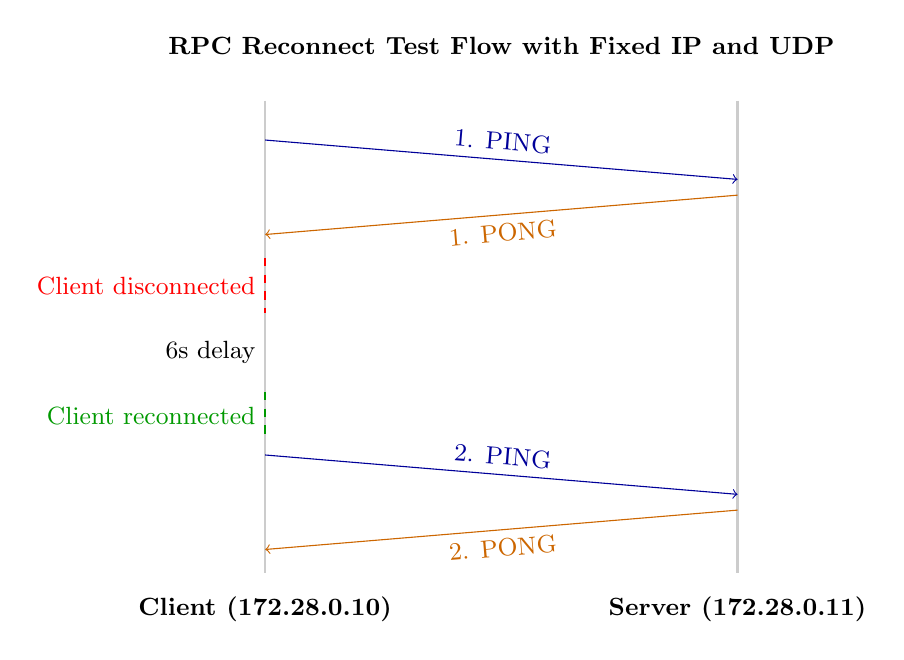
\begin{tikzpicture}[
		timeline/.style={draw=gray!40, thick},
		client/.style={blue!60!black},
		server/.style={orange!80!black},
		event/.style={font=\small, align=left},
		every node/.append style={font=\small}
		]
		
		% Vertical lines for Client and Server
		\draw[timeline] (0,0) -- (0,-6) node[below=0.5em] {\textbf{Client (172.28.0.10)}};
		\draw[timeline] (6,0) -- (6,-6) node[below=0.5em] {\textbf{Server (172.28.0.11)}};
		
		% Events
		% Initial ping
		\draw[->, client] (0,-0.5) -- (6,-1) node[midway, above, sloped] {1. PING};
		\draw[->, server] (6,-1.2) -- (0,-1.7) node[midway, below, sloped] {1. PONG};
		
		% Disconnect
		\draw[dashed, thick, red] (0,-2) -- (0,-2.7);
		\node[event, left] at (0,-2.35) {\textcolor{red}{Client disconnected}};
		
		% Wait period
		\node[event, left] at (0,-3.2) {6s delay};
		
		% Reconnect
		\draw[dashed, thick, green!60!black] (0,-3.7) -- (0,-4.3);
		\node[event, left] at (0,-4.0) {\textcolor{green!60!black}{Client reconnected}};
		
		% Second ping
		\draw[->, client] (0,-4.5) -- (6,-5.0) node[midway, above, sloped] {2. PING};
		\draw[->, server] (6,-5.2) -- (0,-5.7) node[midway, below, sloped] {2. PONG};
		
		% Title
		\node at (3,0.7) {\textbf{RPC Reconnect Test Flow with Fixed IP and UDP}};
		
	\end{tikzpicture}
	\caption{View of the reconnect test: the client disconnects and reconnects}
	\label{fig:rpc_reconnect_timeline}
\end{figure}



\vspace{0.4em}
\begin{table}[H]
	\centering
	\begin{tabular}{@{}lllll@{}}
		\toprule
		\textbf{Component} & \textbf{Role} & \textbf{IP Address} & \textbf{Mode} & \textbf{Response} \\
		\midrule
		rpc\_ping\_server & RPC Server & 172.28.0.11 & network\_udp & PONG \\
		rpc\_ping\_client & RPC Client & 172.28.0.10 & network\_udp & 2×PONG \\
		\bottomrule
	\end{tabular}
	\caption{Setup for RPC reconnect test}
	\label{tab:rpc_reconnect_test}
\end{table}

\vspace{0.5em}
\textbf{Code Examples:}

\vspace{0.4em}
\textbf{Fixed IP assignment in Robot Framework:}

\vspace{0.4em}
The following Robot Framework keyword starts the client and server containers with fixed IP addresses. This ensures consistent addressing across disconnect and reconnect steps.

\vspace{0.4em}
\begin{lstlisting}[style=cppstyle, caption={Starting containers with fixed IPs}, label={lst:rf_start_with_ip}, captionpos=b]
 Start Container With IP   rpc_server   ${IMAGE}   server
 ...    network=${NETWORK}    ip=${SERVER_IP}
 
 Start Container With IP   rpc_client   ${IMAGE}   client
 ...    network=${NETWORK}    ip=${CLIENT_IP}
\end{lstlisting}

\newpage
\vspace{0.4em}
\textbf{Simulating disconnect and reconnect:}

\vspace{0.4em}
This part disconnects the client from the network and reconnects it later with the same IP. It simulates a temporary connection failure during runtime.

\vspace{0.4em}
\begin{lstlisting}[style=cppstyle, caption={Simulating network disconnect and reconnect}, label={lst:rf_disconnect_reconnect}, captionpos=b]
 Disconnect Container From Network   rpc_client   ${NETWORK}
 Sleep    7s
 Reconnect Container To Network    rpc_client    ${NETWORK}
                                   ${CLIENT_IP}
\end{lstlisting}


\vspace{0.3em}
The client performs two RPC calls: one before and one after simulated network loss (Listing~\ref{lst:rpc_reconnect_client}).

\begin{lstlisting}[style=cppstyle, caption={Client performs reconnect and second RPC call}, label={lst:rpc_reconnect_client}, captionpos=b]
 int pong_counter = 0;
 int error = call_rpc(client, "Initial", pong_counter);
 std::this_thread::sleep_for(std::chrono::seconds(8));
 error += call_rpc(client, "Reconnect", pong_counter);
 return (pong_counter >= 2 && error == 0) ? 0 : 1;
\end{lstlisting}

\vspace{0.5em}
\textbf{Evaluation:}

\vspace{0.4em}
This test checks how well the eCAL RPC system can handle changing network conditions. By disconnecting the client from the Docker network for a short time, it simulates a temporary network failure. After reconnecting, the client tries to call the server again using the same IP address.

\vspace{1em}
eCAL uses service discovery to manage RPC connections. In the case of UDP, this discovery is usually based on multicast messages that are sent across the network. For this to work correctly after a reconnect, the system needs to keep using the same network interface and IP address. The fixed IPs in this test make sure that the server still recognizes the client after reconnecting.

\vspace{1em}
This setup is similar to real use cases, for example in embedded systems where network connections can drop and come back. The test shows that eCAL can recover from such a disconnection. Both calls (before and after the network drop) are successful, which means that the client could reconnect and the server was still available. This gives confidence that eCAL RPC over UDP multicast can be used in systems where short network problems may happen.


\subsection{Automation and Repeatability}

A key objective of the integration test design is to ensure that all tests can be executed in a fully automated and repeatable manner. Automation is important for enabling reliable regression testing, especially in the context of continuous integration and deployment (CI/CD).

\vspace{0.9em}
In this project, the test cases are implemented using the Robot Framework and can be executed with a single command:

\begin{verbatim}
	robot --outputdir results network_crash.robot
\end{verbatim}

\vspace{0.5em}
This command runs the specified test and stores all result files in the \texttt{results} directory. The following artifacts are automatically generated after each run:

\begin{itemize}
	\item \textbf{log.html} – A detailed execution log, including all console output
	\item \textbf{report.html} – A summary report presenting the test results in a structured format
	\item \textbf{output.xml} – A machine readable file with raw test data for further processing or CI integration
\end{itemize}

\vspace{0.9em}
To ensure automated and consistent test execution, the tests are fully integrated into GitHub Actions. This platform offers native support for defining CI workflows directly in the repository using YAML configuration files. The integration allows tests to be triggered automatically in the following scenarios:

\begin{itemize}
	\item After each push to the main repository (continuous integration)
	\item Manually via the GitHub Actions web interface
\end{itemize}

\vspace{0.5em}
Test results are stored and deployed via GitHub Pages, enabling direct access to all test reports through a structured web interface. Each test run is timestamped and, if available, linked to the triggering commit, ensuring traceability across test history.

\vspace{0.5em}
The overall interaction between the main repository and the ecal-test-suite is illustrated in the following diagram:

\vspace{1em}
\begin{center}
	\begin{tikzpicture}[
		node distance=1.8cm and 3cm,
		repo/.style={rectangle, draw=blue!60, fill=blue!10, very thick, minimum width=3cm, minimum height=1cm},
		action/.style={rectangle, draw=gray!80, fill=gray!20, minimum width=3.8cm, text width=3.5cm, align=center},
		arrow/.style={->, thick},
		status/.style={rectangle, draw=green!50!black, fill=green!10, minimum width=3.8cm, text width=3.5cm, align=center},
		web/.style={rectangle, draw=orange!80!black, fill=orange!10, minimum width=3.8cm, text width=3.5cm, align=center}
		]
		
		\node[repo] (repo1) {eCAL Repository};
		\node[action, below=of repo1] (trigger) {Trigger: On Push to master};
		\node[action, below=of trigger] (dispatch) {repository\_dispatch to Tests};
		
		\node[repo, right=5.5cm of repo1] (repo2) {ecal-test-suite Repository};
		\node[action, below=of repo2] (ci) {CI Run: Docker + Robot Framework};
		\node[web, below=of ci] (pages) {Reports deploy to GitHub Pages};
		
		\node[status, left=0.8cm of repo2] (feedback) {Status back to eCAL\\(success/failure)};
		
		\draw[arrow] (repo1) -- (trigger);
		\draw[arrow] (trigger) -- (dispatch);
		\draw[arrow] (dispatch) -- (repo2);
		\draw[arrow] (repo2) -- (ci);
		\draw[arrow] (ci) -- (pages);
		\draw[arrow] (ci.west) -- (feedback.east);
		\draw[arrow] (feedback) -- (repo1);
		
	\end{tikzpicture}
	\captionof{figure}{Interaction between the main eCAL repository and the ecal-test-suite for automated integration testing}
	\label{fig:ci_architecture_overview}
\end{center}

The corresponding source code, test logic, and CI configuration are available in the public \texttt{ecal-test-suite} repository~\cite{ecal_test_suite_repo}. All results are automatically published to GitHub Pages~\cite{ecal_test_suite_ghpages} for transparency and accessibility.

\vspace{1em}
This architecture ensures that integration tests are decoupled from the main development repository, yet fully synchronized through GitHub's event-based automation mechanisms. Status feedback, report visibility, and reproducibility are guaranteed at every stage of the workflow.

\vspace{1em}
In addition, the use of Docker for test isolation ensures high portability and reproducibility. Tests can be executed in local development environments, on cloud-based runners, or within virtualized test infrastructure—independent of the host system configuration. This improves consistency across different environments and reduces the likelihood of platform-specific errors.

\clearpage
\subsection{Visualization of Test Results}

The successful automation of integration tests is only effective if test results can be accessed, interpreted, and compared efficiently. Therefore, this project includes a visual reporting system that makes all results available via the browser.

\vspace{0.9em}
After each test execution, GitHub Actions deploys the generated reports to the \textbf{GitHub Pages} section of the test repository. The following figure shows the structured web interface, where all test runs are listed by timestamp. If available, the commit hash that triggered the test run is also displayed for traceability.

\begin{figure}[H]
	\centering
	\includegraphics[width=\textwidth]{Images/github_pages_overview.png}
	\caption{Test report overview hosted on GitHub Pages}
	\label{fig:gh_pages_overview}
\end{figure}

\vspace{0.5em}
Clicking on a specific test entry opens the detailed Robot Framework report. This report contains structured sections with statistics, test case results, execution logs, and console output. The clear layout enables quick identification of failed tests and debugging of communication problems.

\begin{figure}[H]
	\centering
	\includegraphics[width=\textwidth]{Images/robot_report_example.png}
	\caption{Detailed Robot Framework report for a test run}
	\label{fig:robot_report}
\end{figure}

\vspace{0.5em}
This visualization not only improves transparency and accessibility but also enables historical comparisons of test outcomes over time. Developers and reviewers can quickly identify regressions or improvements in communication stability and test coverage.

\newpage
\subsection{Summary}

This chapter presented the design, implementation, and execution of a modular integration test system for the eCAL middleware. By combining Docker based process isolation with the flexible automation capabilities of Robot Framework, it was possible to validate key properties of publish-subscribe communication in a controlled and reproducible environment.

\vspace{1em}
The selected test cases focused on core functionalities such as reliable message delivery, multi-node communication, and fault tolerance under crash or failure conditions. Most scenarios were tested across all five supported eCAL transport modes, these are shared memory (SHM), UDP, and TCP in both local and network configurations. This ensured broad coverage of both common and edge-case communication patterns.

\vspace{1em}
Code examples demonstrated how publishers, subscribers, and test logic are implemented and configured, while structured success criteria and exit codes provided clear validation of expected behavior. The test infrastructure also proved effective in simulating failure scenarios such as process crashes and message loss, confirming the robustness and resilience of the eCAL middleware.

\vspace{1em}
A notable insight from these tests is the performance resilience trade off introduced by advanced features like Zero-Copy SHM. While this mode improves throughput by eliminating memory copies, it also increases inter-process coupling and may compromise fault isolation if a subscriber crashes during message access. Future deployments should carefully assess whether the performance benefits of Zero-Copy justify its potential stability risks.

\vspace{1em}
The framework is already equipped to be extended with further test categories. For example, future work could include RPC based communication, service availability tests, and metrics such as round-trip time. Moreover, integration into CI/CD pipelines would enable automatic regression testing during development and deployment.

\vspace{1em}
In conclusion, the developed test system successfully demonstrates how integration tests can be used not only for functional verification but also to explore system behavior under realistic and adverse conditions. It provides a solid foundation for continuous validation of middleware functionality in research, development, and production contexts.


